\documentclass{article}
\usepackage[utf8]{inputenc}
\usepackage[margin=1in]{geometry}
\usepackage{hyperref}
\usepackage{graphicx}

\title{Parallel Programming - MPI Project}
\author{Kamal Aghayev\\
		\texttt{kamal.aghayev@ufaz.az}}
\date{\today}

\begin{document}

\maketitle

\section{Introduction}
	Message Passing Interface (MPI) is a standardized and portable message-passing standard designed by a group of researchers from academia and industry to function on a wide variety of parallel computing architectures.
	The goal of the current project is to develop two distinct programs that run with MPI and analyze their behaviour when used on a machine and on several machines remotely.
	
\section{Ping Pong}
	The idea of the Ping Pong program is to send messages from a machine to another repeteadly many times. Below you may see the graph that shows the dependency of the message transfer rate on the length of the message sent (see Fig. \ref{fig:ping_pong}).
	\begin{figure}[htbp]
    	\centering
    	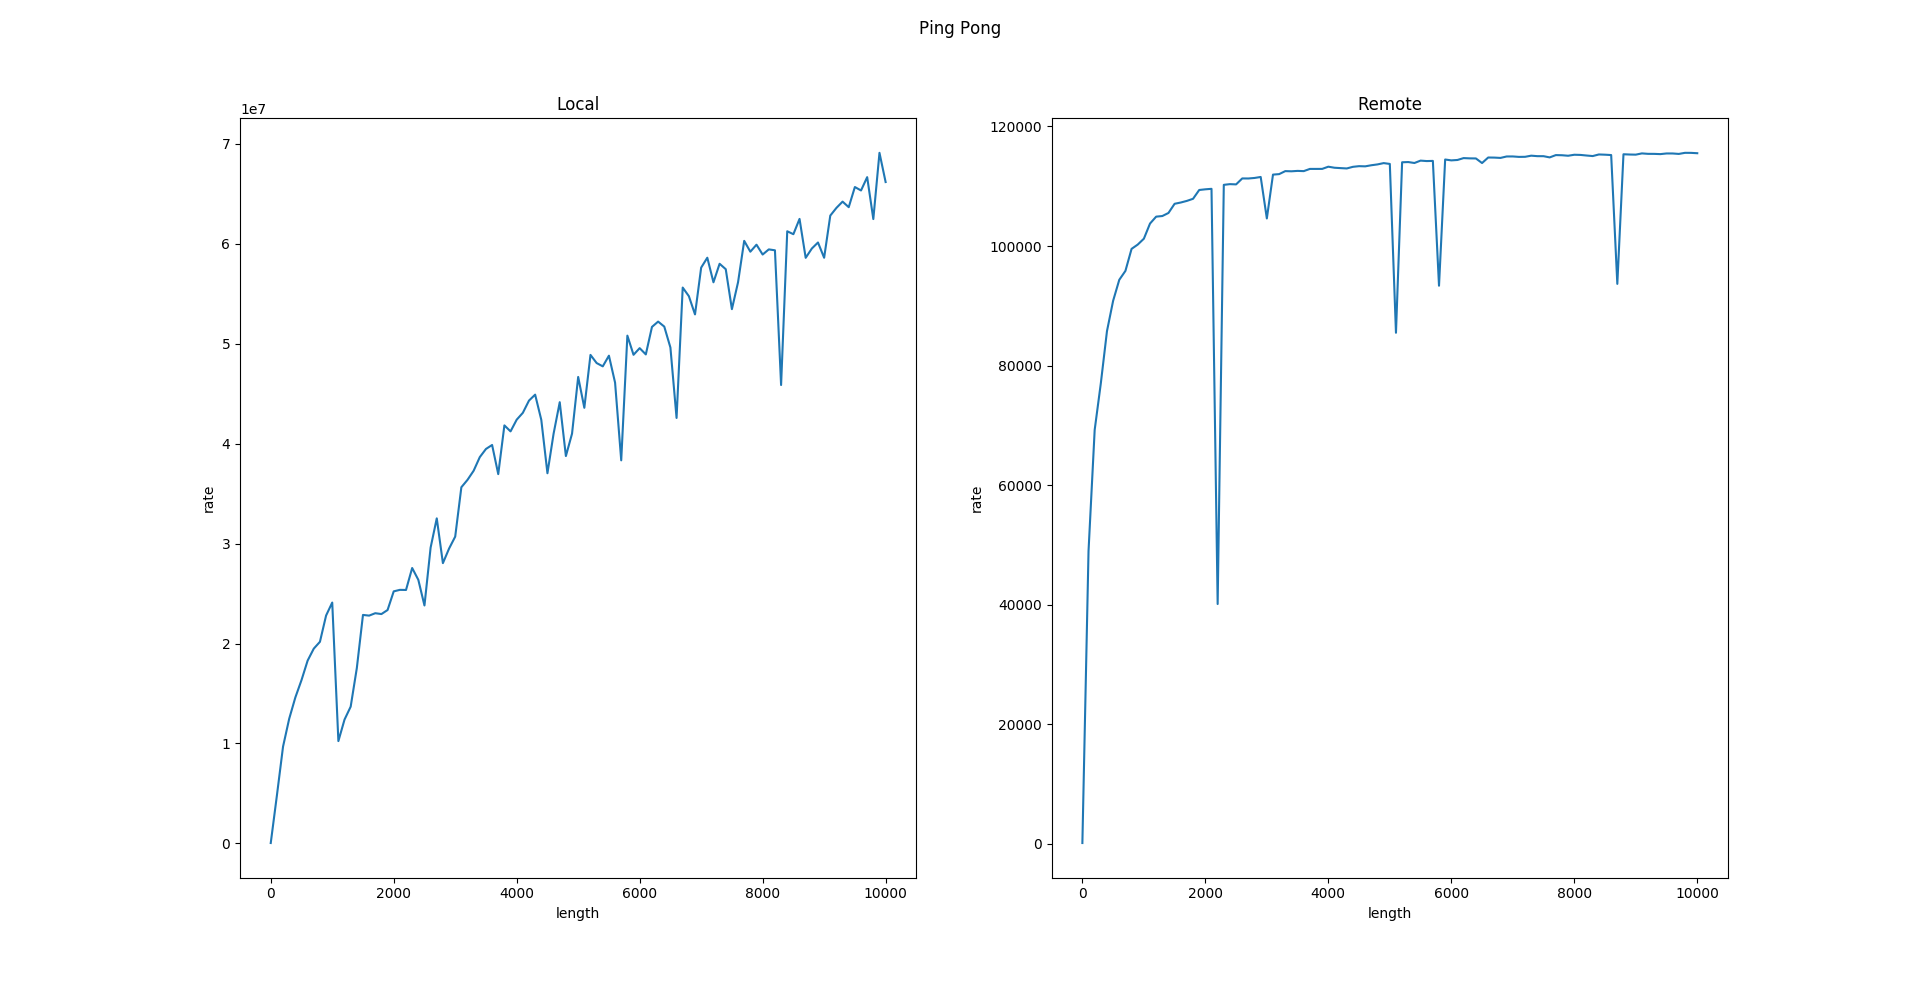
\includegraphics[width=\textwidth]{ping_pong.png}
    	\caption{Ping Pong}
    	\label{fig:ping_pong}
	\end{figure}

	As can be seen on the plot, the transfer rate in local is much higher than that remotely. Moreover, the shape of the plot differs in two different modes: in the local the dependency is strictly linear, while in the remote the small message length is sent with a low transfer rate, while getting bigger the transfer rate starts increasing fast but then the dependency becomes linear.
	
	
\section{Merge Sort}

	\subsection{Interface}
		Since the source code for this part of the project has to be provided by us, I developed my own version of the program. The algorithm of the program is as follows:
		\begin{enumerate}
			\item The input array is spread to all the machines and each machine receives $\frac{N}{n}$ elements of an array, where $N$ is the size of an array, and $n$ is the number of machines.
			\item Each machine uses quick sort on the part of the array it received.
			\item 
				\begin{itemize}
					\item All the machines start to send the $i$\textsuperscript{th} element of the sorted array to the machine with 0 rank and receives the response. Response is either 0, which means that the number is not used in the current step, or the response is 1, which means that the current value is the smallest sent, so that it is included in the merged array. Then the counter $i$ is incremented and the process continues until $i < \frac{N}{n}$, i.e. all the lements of the current machine are used.
					\item The machine with 0 rank starts receiving the values from other machines and compares these values, including its own value. The machine with the smallest value receives 1 as a response, while other machines receive 0. The process continues until the merged array is not full.
				\end{itemize}							
		\end{enumerate}
		
		This interface, of course, is very bad, but it represents how the bad interface between several machines may lead to big problems. This happens because there are a lot of messages passing between machines, while they are very costful. The best decision would be to send all the sorted values at once decreasing number of messages sent between processes to the minimum, but this was not the goal of the project, so I decided that practical experience of how catastrophic the bad interface may be is much valuable.
		
	\subsection{Local}
		Below you may see the graph that shows the dependency of the time needed to sort the array on the size of an array (see Fig. \ref{fig:merge_local}).
		\begin{figure}[htbp]
    		\centering
    		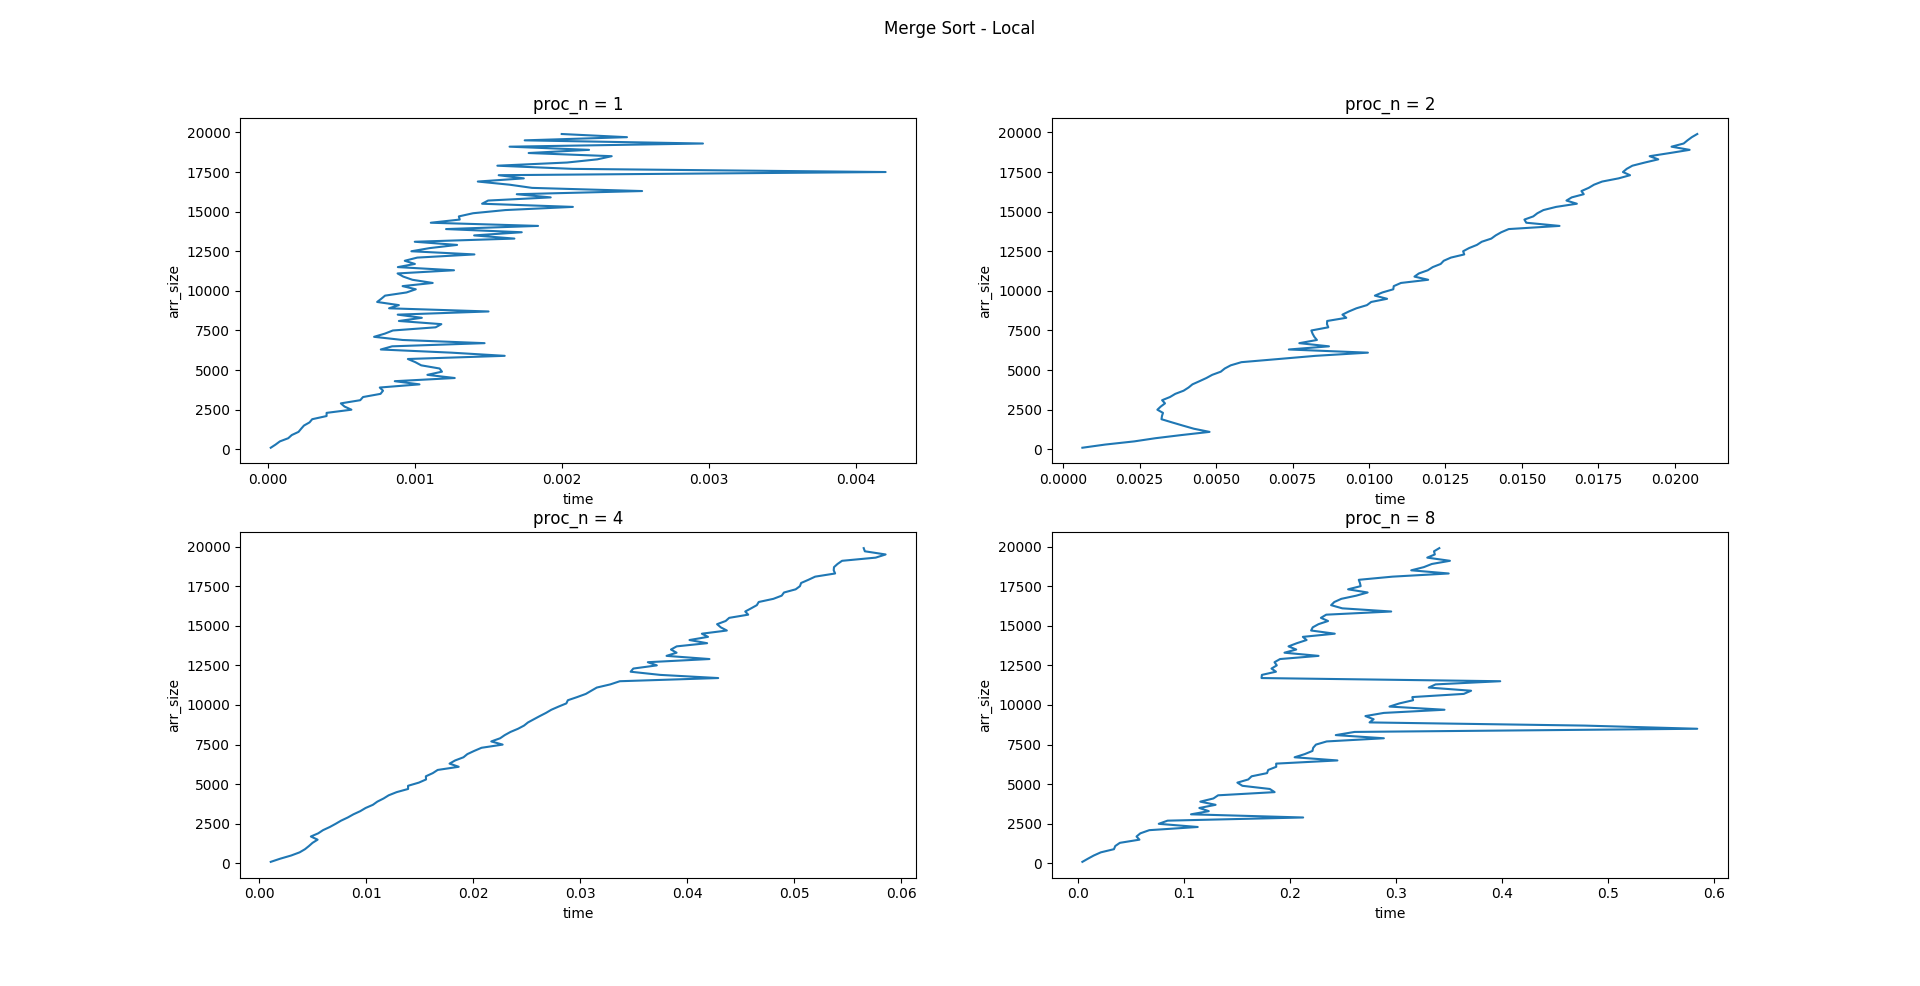
\includegraphics[width=\textwidth]{merge_local.png}
    		\caption{Merge Sort. Local}
    		\label{fig:merge_local}
		\end{figure}
		
		It can be easily noticed that with higher number of machines, the time needed to sort the array increases significantly due to the bad interface.
	
	\subsection{Remote}
		Due to the technical problems, I was not able to run the same program in a remote mode; however, all the job to run was done. The only remaining part was to run the program in remote, collect all the output data in the file and give the file as an input to the plotting script which would show the plot. I tried to run this program at home; however, I could not succed due to the different versions of the OS and \texttt{mpicc/mpirun}. And I was not able to go to the SP2 building due to the tough schedule.
		
		
		
		
		
		
		

\end{document}